%%-*-latex-*-

\documentclass[wide]{slides}

% Language
%
\usepackage{hyphenat}          % \hyp{} is a breakable dash

\frenchspacing  % Follow French conventions after a period

% Maths
%
\usepackage{stmaryrd}

% Graphics
%
\usepackage{graphicx}

% Miscellanea
%
\usepackage{varioref}  % Qualifying references with page numbers

% New environments and commands
%
../TeX/commands.tex

%---------------------------------------------------------------
% Document
%
\maintitle{A Theory of Programming}
\mainauthor{\textbf{Christian Rinderknecht}\\
  {\small\url{Christian.Rinderknecht@nomadic-labs.com}}\\
\Nomadic}
\confname{Tezos Masterclass}
\confshortname{Tezos}
\confdate{20 October 2018}

\begin{document}

\maketitle

\begin{slide}
  \title{Introduction}

  \begin{itemize}

    \item This series of lectures proposes a stepwise introduction to
      \textbf{functional programming} and the analyses to write
      reliable and efficient software.

    \item The theoretical background of functional languages is formal
      logic, where mathematical functions are the main building block.

    \item This close link with formal logic implies that the meaning
      of functional programs can often be made very precise.

    \item It is a good framework to get a sense of \textbf{static
      analyses}, and, as such, it stands a prominent place in the
      field of formal methods and \textbf{compiler construction}.

    %% \item This lecture is concerned with \textbf{programming in the
    %%   small}, not with solving any realistic problems yet.

  \end{itemize}
\end{slide}

\begin{slide}
  \title{Introduction}

  \begin{itemize}

    \item In a later lecture, we will learn a specific programming
      language called \textbf{\OCaml}, enabling you to put in practice
      what you have learnt.

    \item \OCaml is used for the core development of the \Tezos
      \textbf{blockchain}.

    \item Most textbooks and courses on \OCaml propose a traditional
      approach: basic concepts, data structures, algorithms.

    \item Here, we aim more at illustrating the kind of software
      \Tezos uses \OCaml for, in particular, compiler construction.

    \item This first lecture is not specific to \OCaml and is
      theoretical because it introduces many concepts that are used in
      functional programming and compiler construction.

  \end{itemize}

\end{slide}

\begin{slide}
  \title{String rewriting}

  \begin{itemize}

    \item Let us consider a string of white and black beads, like
      \(\circ \bullet \bullet \bullet \circ \circ \bullet\), and a
      one-player game whose unique move consists in replacing two
      adjacent beads with only one according to the rules
      \begin{equation*}
        \bullet \; \circ   \xrightarrow{\alpha} \bullet\qquad\qquad
        \circ   \; \bullet \xrightarrow{\beta} \bullet\qquad\qquad
        \bullet \; \bullet \xrightarrow{\gamma} \circ
      \end{equation*}

    \item The rules~\(\alpha\), \(\beta\)~and~\(\gamma\) make up a
      simple \textbf{string\hyp{}rewriting system}.

    \item Rules \(\alpha\)~and~\(\beta\) can be conceived
      as:\\ \emph{A black bead absorbs the white bead next to it.}

    \item The goal of this game is to end up with as few beads as
      possible, so our example may lead to the \textbf{rewrites}
      \begin{equation*}
        \circ \bullet \bullet \, \fbox{\(\bullet\; \circ\)} \circ
        \bullet \xrightarrow{\alpha} \circ \bullet \bullet \,
        \fbox{\(\bullet\; \circ\)} \; \bullet
        \xrightarrow{\alpha} \fbox{\(\circ \; \bullet\)} \;
        \bullet \bullet \,\bullet \xrightarrow{\beta} \bullet
        \bullet \, \fbox{\(\bullet \; \bullet\)}
        \xrightarrow{\gamma} \bullet \, \fbox{\(\bullet \;
          \circ\)} \xrightarrow{\alpha} \fbox{\(\bullet \;
          \bullet\)} \xrightarrow{\gamma} \circ
      \end{equation*}

      \medskip
      \noindent where the part of the string to be rewritten next is
      framed.

  \end{itemize}

\end{slide}

\begin{slide}
  \title{Normal forms and termination}

  \begin{itemize}

    \item Other compositions of the rules lead to the same
      result~\(\circ\) as well. Some others bring all\hyp{}white or
      all\hyp{}black strings, like \(\circ \, \circ\) and~\(\bullet\).

    \item Strings that can not be further rewritten, or
      \textbf{reduced}, are called \textbf{normal forms}.

    \item We may wonder whether all strings have a normal form, and,
      if so, if it is unique and, furthermore, if it is either
      all\hyp{}white or all\hyp{}black.

    \item First, let us note that the system is \textbf{terminating},
      that is, there is no infinite chain of rewrites, because the
      number of beads strictly decreases in all the rules.

    \item This is not a necessary condition in general, for instance,
      \(\circ \; \bullet \xrightarrow{\beta} \bullet \circ
      \circ\) would preserve termination because the composition
      \(\beta\alpha\alpha\) would be equivalent to the original
      rule~\(\beta\).

    \item In particular, this means that any string has a normal form.

  \end{itemize}
\end{slide}

\begin{slide}
  \title{Invariants}

  \begin{itemize}

    \item Second, notice how the parity of the number of black beads
      is \textbf{invariant} through each rule and how there is no
      rewrite rule for two adjacent white beads.

    \item Therefore, if there are \(2p\) initial black beads, then
      composing rules \(\alpha\)~and~\(\beta\) lead to an
      all\hyp{}black string, which can be reduced by applying
      rule~\(\gamma\) to contiguous pairs of beads into an
      all\hyp{}white string made of \(p\)~beads.

    \item Otherwise, the same all\hyp{}black string can be reduced by
      applying alternatively \(\gamma\)~and~\(\beta\) on the left end
      or \(\gamma\)~and~\(\alpha\) on the right end,
      yielding~\(\circ\).

    \item Similarly, if there is an initial odd number of black beads,
      we always end up with one black bead.

  \end{itemize}

\end{slide}

\begin{slide}
  \title{Confluence}

  \begin{itemize}

    \item Consequently, normal forms are not unique.

    \item A simple example is
      \begin{equation*}
        \circ \circ \xleftarrow{\gamma} \bullet \bullet \circ
        \xrightarrow{\alpha} \bullet \bullet \xrightarrow{\gamma}
        \circ
      \end{equation*}

    \item Systems where normal forms are unique are
      \textbf{confluent}.

    \item If we think of a rewrite step as an elementary computation,
      it becomes clear that confluence is a desirable property for
      carrying out computations, as we would expect, for instance, an
      arithmetic expression to have the same value no matter the order
      of the small steps.

    \item A systemic order of rule application is called a
      \textbf{reduction strategy}.

  \end{itemize}

\end{slide}

\begin{slide}
  \title{Completing a system}

  \begin{itemize}

    \item We can obtain confluence by adding the rule~\(\delta\):
      \begin{equation*}
        \bullet \; \circ   \xrightarrow{\alpha} \bullet\qquad\qquad
        \circ   \; \bullet \xrightarrow{\beta} \bullet\qquad\qquad
        \bullet \; \bullet \xrightarrow{\gamma}
        \circ\qquad\qquad
        \circ\; \circ \xrightarrow{\delta} \circ
      \end{equation*}
      the result of the game is always one bead, whose colour depends
      on the original parity of the black beads as before.

    \item To see why, let us consider first that two
      non\hyp{}overlapping parts of a string can be rewritten in
      parallel, so they are not a concern.

    \item The interesting cases occur when two applications of rules
      (maybe of the same rule) lead to different strings because they
      do overlap. For instance,
      \begin{equation*}
        \circ \, \circ \xleftarrow{\gamma} \bullet \bullet
        \circ \xrightarrow{\alpha} \bullet \, \bullet
      \end{equation*}

    \item The important point is that \(\circ \, \circ\) and \(\bullet
      \, \bullet\) can be rewritten into~\(\circ\) at the next step by
      \(\delta\)~and~\(\gamma\), respectively.

  \end{itemize}

\end{slide}

\begin{slide}
  \title{Critical pairs}

  \begin{itemize}

    \item In general, what matters is that all pairs of strings
      resulting from the application of overlapping rules, called
      \textbf{critical pairs}, can be rewritten to the same string:
      they are \textbf{joinable}.

    \item In our example, all interactions occur on substrings made of
      three beads, so we must examine eight cases:
      \begin{center}
        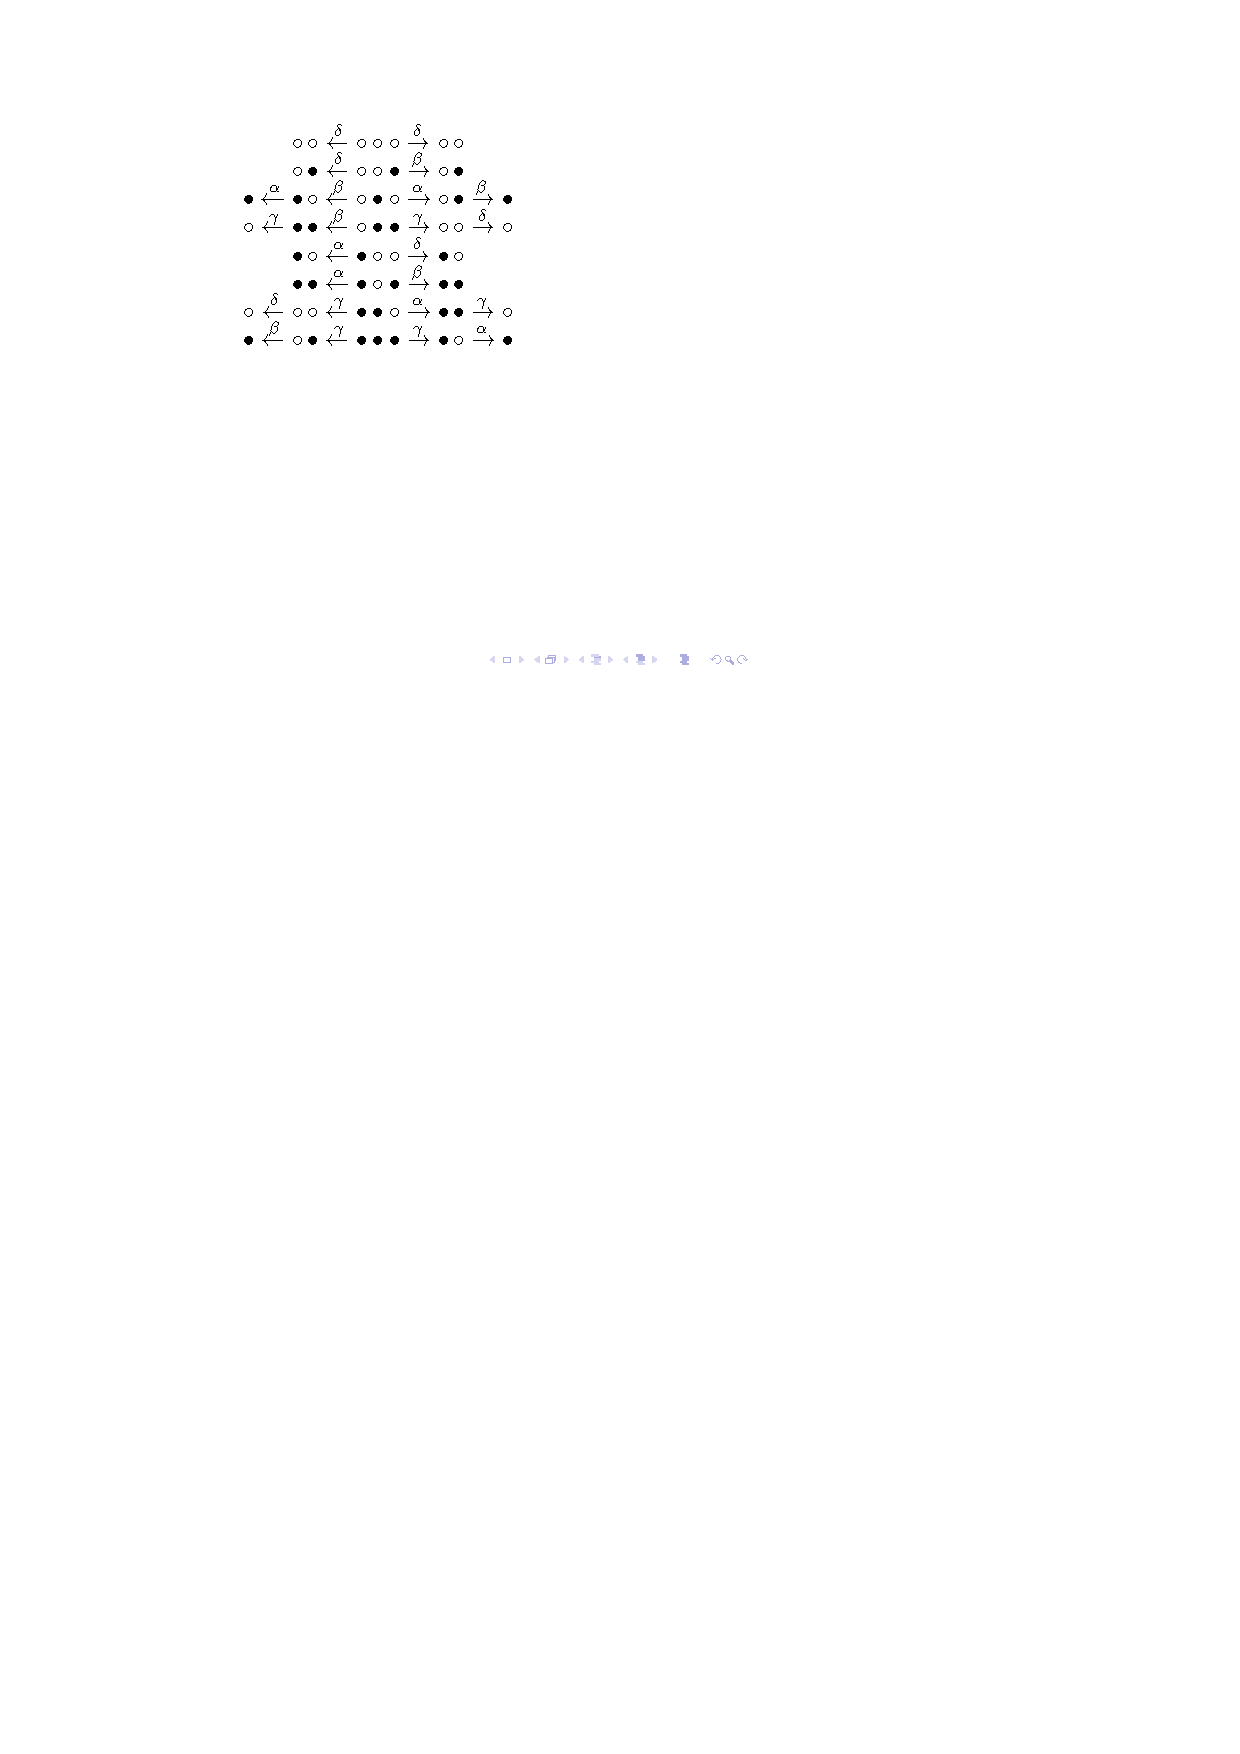
\includegraphics[trim=7cm 55mm 7cm 2mm]{bullets.pdf}
      \end{center}

    \item In all the cases, the divergences are joinable in one step
      at most.

  \end{itemize}

\end{slide}

\begin{slide}
  \title{Local confluence}

  \begin{itemize}

    \item If all critical pairs are joinable after a divergence in one
      ore more rewrites, the system is \textbf{locally confluent}.

    \item Moreover, if the system is also terminating, then
      \textbf{every} string has exactly \textbf{one} normal form (a
      strong property entailing confluence).

    \item Sometimes, as seen previously, a non\hyp{}confluent system
      can be completed to become confluent, via a \textbf{completion
        procedure}.

      \item In the case of terminating systems, one of such
        semi\hyp{}decision procedures is the Knuth\hyp{}Bendix
        algorithm.
  \end{itemize}

\end{slide}

\begin{slide}
  \title{Ground and linear rewrite systems}

  \begin{itemize}

    \item The system we defined is \textbf{ground}, that is, it
      involves no variables.

    \item These allow a finite system to denote an infinite number of
      ground rules if variables range over infinite sets, or simply,
      they reduce the size of rewrite systems.

    \item For instance, our continued example is equivalent to
      \begin{equation*}
        \bullet \; \circ \xrightarrow{\alpha} \bullet
        \qquad\qquad
        \circ \; x \xrightarrow{\beta+\delta} x
        \qquad\qquad
        \bullet \; \bullet \xrightarrow{\gamma} \circ
      \end{equation*}

    \item If we accept multiple occurrences of a variable on the
      left\hyp{}hand side of a rule, a so\hyp{}called \textbf{non
        left\hyp{}linear rule}, we can further decrease the size of
      the system:
      \begin{equation*}
        x  \; x \xrightarrow{\gamma+\delta} \circ\qquad\qquad
        x  \; y \xrightarrow{\alpha+\beta} \bullet
      \end{equation*}

  \end{itemize}
\end{slide}

\begin{slide}
  \title{Ordered rewrite systems}

  \begin{itemize}

    \item Notice that there is now an implicit order over the rules:
      the rule \(\gamma+\delta\) must be examined first for a
      \textbf{match} with a part of the current string, because it is
      included in the second (set \(x=y\) in \(\alpha+\beta\)).

    \item Non\hyp{}linear systems are equational theories due the
      implicit equality on substructures, which is complex: we will
      limit ourselves to \textbf{linear systems}.

    \item In general, the order in which the rules are written on the
      page is their \textbf{logical order}.

    \item Moreover, let us remark that the system does not specify
      that \(x\)~must either be~\(\circ\) or~\(\bullet\): this should
      be stated nevertheless somewhere else.

    \item Generally speaking, this means that the \textbf{type} of the
      variables has to be defined elsewhere or inferred from the
      variable uses.

      \item We will return to that topic about \OCaml.

  \end{itemize}
\end{slide}

\begin{slide}
  \title{Term rewriting}

  \begin{itemize}

    \item More general are the \textbf{term\hyp{}rewriting systems},
      where a \textbf{term} is a mathematical object built on tuples,
      integers and variables.

    \item Let us consider the following totally ordered system:
      \begin{align*}
        (0,m) &\xrightarrow{1} m\\
        (n,m) &\xrightarrow{\smash 2} (n-1, n \times m)\\
        n     &\xrightarrow{\smash 3} (n,1)
      \end{align*}

      \item Arithmetic operators \((-)\)~and~\((\cdot)\) are defined
        out of the system and \(m\)~and~\(n\) are variables denoting
        natural numbers.

      \item Would the rules not be ordered as they are
        actually laid out, the second rule would match any
        pair. Instead, it can be assumed that \(n \neq 0\) when
        matching with it.

      \item The last rule is to be tried last, as it matches all
        terms.

  \end{itemize}
\end{slide}

\begin{slide}
  \title{Transitive closures}

  \begin{itemize}

    \item We can easily see that all the compositions of rewrites
      starting with a natural number~\(n\) end with the factorial
      of~\(n\):
      \smallskip
      \begin{equation*}
        n \xrightarrow{3} (n,1)
        \xrightarrow{2} \dots
        \xrightarrow{2} (0,n!)
        \xrightarrow{1}
        n!, \quad \text{for \(n \in \mathbb{N}\)}.
      \end{equation*}

    \item Let us note \((\xrightarrow{n})\) the composition of
      \((\rightarrow)\) repeated \(n-1\)~times:
      \begin{align*}
        (\xrightarrow{1})   &:= (\rightarrow)\\
        (\xrightarrow{\smash{n+1}}) & :=
        (\rightarrow) \circ (\xrightarrow{\smash{n}}),
        \quad\text{with \(n > 0\)}.
      \end{align*}

    \item The \textbf{transitive closure} of \((\rightarrow)\) is
      defined as
      \begin{equation*}
        (\twoheadrightarrow) := \bigcup_{i >
          0}{(\xrightarrow{i})}.
        \end{equation*}

    \item The factorial function coincides with the transitive closure
      of \((\rightarrow)\): \(n \twoheadrightarrow
      n!\).

    \item Let \((\xrightarrow{*})\) be the
      reflexive\hyp{}transitive closure of \((\rightarrow)\), that is,
      \begin{equation*}
        (\xrightarrow{*}) := (=) \cup (\twoheadrightarrow).
      \end{equation*}

  \end{itemize}

\end{slide}

\begin{slide}
  \title{Functions}

  \begin{itemize}

    \item A confluent system defines a \textbf{partial function}.

    \item If the system is also terminating, we get a
      \textbf{function}.

    \item We can name functions: for example, \(\fun{c}(1,
      \fun{d}(n))\)~is a term constructed with \textbf{function names}
      \fun{c}~and~\fun{d}, as well as variable~\(n\).

    \item A tuple tagged with a function name, like \(\fun{f}(x,y)\),
      is called a \textbf{function call}.

    \item The components of the tuples are then called
      \textbf{arguments}, for example \(\fun{d}(n)\) is the second
      argument of the call \(\fun{c}(1, \fun{d}(n))\).

    \item It is possible for a function call to hold no arguments,
      like \(\fun{d}()\).

    \item We restrict the left\hyp{}hand sides of rules to be function
      calls.

  \end{itemize}

\end{slide}

\begin{slide}
  \title{Trees}

  \begin{itemize}

    \item The topological understanding of a function call or a tuple
      is the finite \textbf{tree}.

    \item A tree is a hierarchical layout of information, for example:
      \begin{center}
        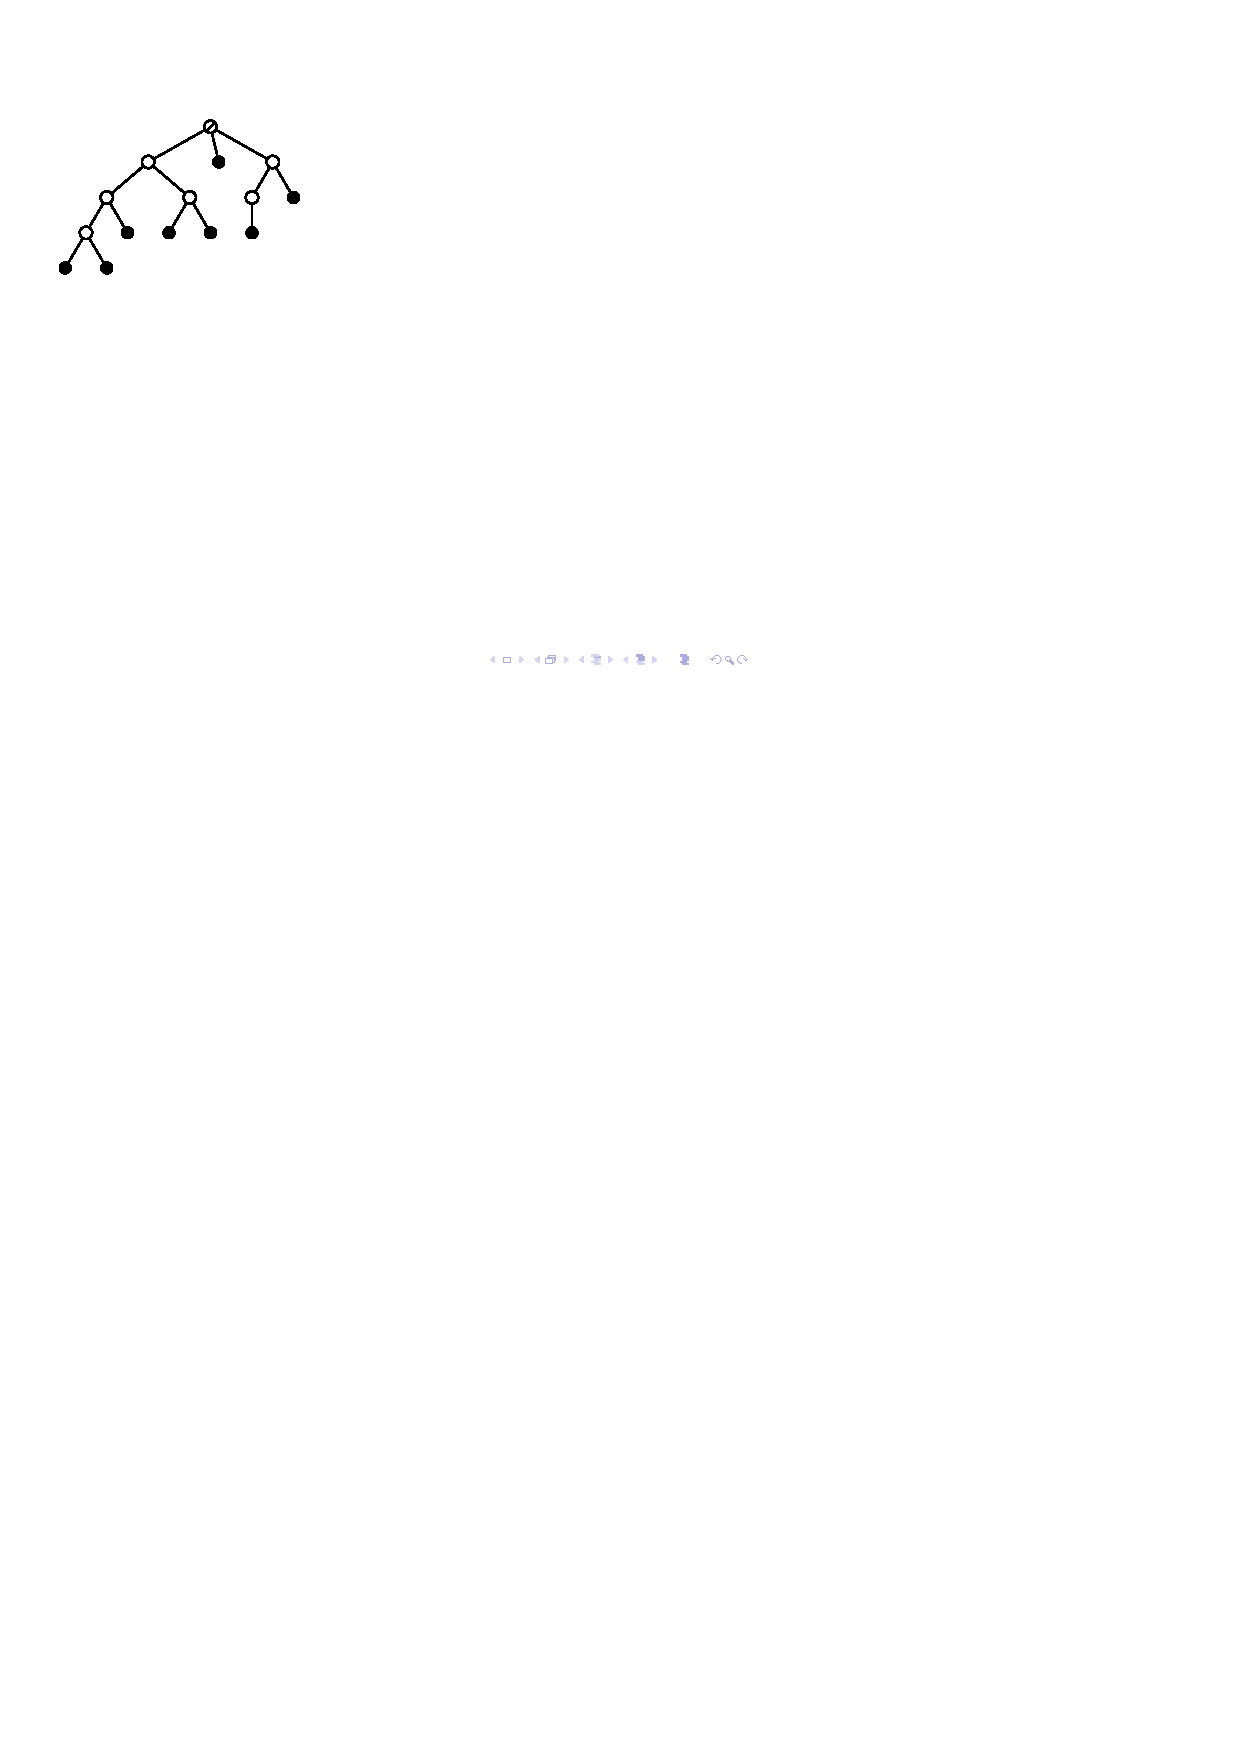
\includegraphics[trim=5mm 6cm 75mm 2mm]{tree_for_term.pdf}
      \end{center}

    \item The disks are called \textbf{nodes} and the segments which
      connect two nodes are called \textbf{edges}. The topmost node
      (with a diameter) is called the \textbf{root} and the bottommost
      ones (\(\bullet\)) are called the \textbf{leaves}. All nodes
      except the leaves are seen to downwardly connect to some other
      nodes, called \textbf{children}. Upwardly, each node but the
      root is connected to another node, called its \textbf{parent}.

  \end{itemize}

\end{slide}

\begin{slide}
  \title{Trees}

  \begin{itemize}

    \item \textbf{Trees are pervasive} in informatics, especially in
      functional programming, but not only.

    \item Structured documents, like books, articles, and web pages,
      are composed of chapters, sections, paragraphs, figures,
      appendices, indices, etc.

    \item The occurrences of these components are mutually
      constrained; for instance, it is understood that a section is
      part of a chapter and that appendices are located at the end of
      a document.

    \item This hierarchical layout is meant to facilitate reading, and
      it supports the search for specific items of information.

    \item When considering computer systems, these data must be
      uniformly encoded by means of a formal language.

  \end{itemize}

\end{slide}


\begin{slide}
  \title{Terms as trees}

  \begin{itemize}

    \item Trees can be used to depict terms as follows. A function
      call is a tree whose root is the function name and the children
      are the trees denoting the arguments.

    \item A tuple can be considered as having an invisible function
      name represented by a node with a period (\texttt{.}) in the
      tree, in which case the components of the tuple are its
      children. For example,
      \begin{center}
        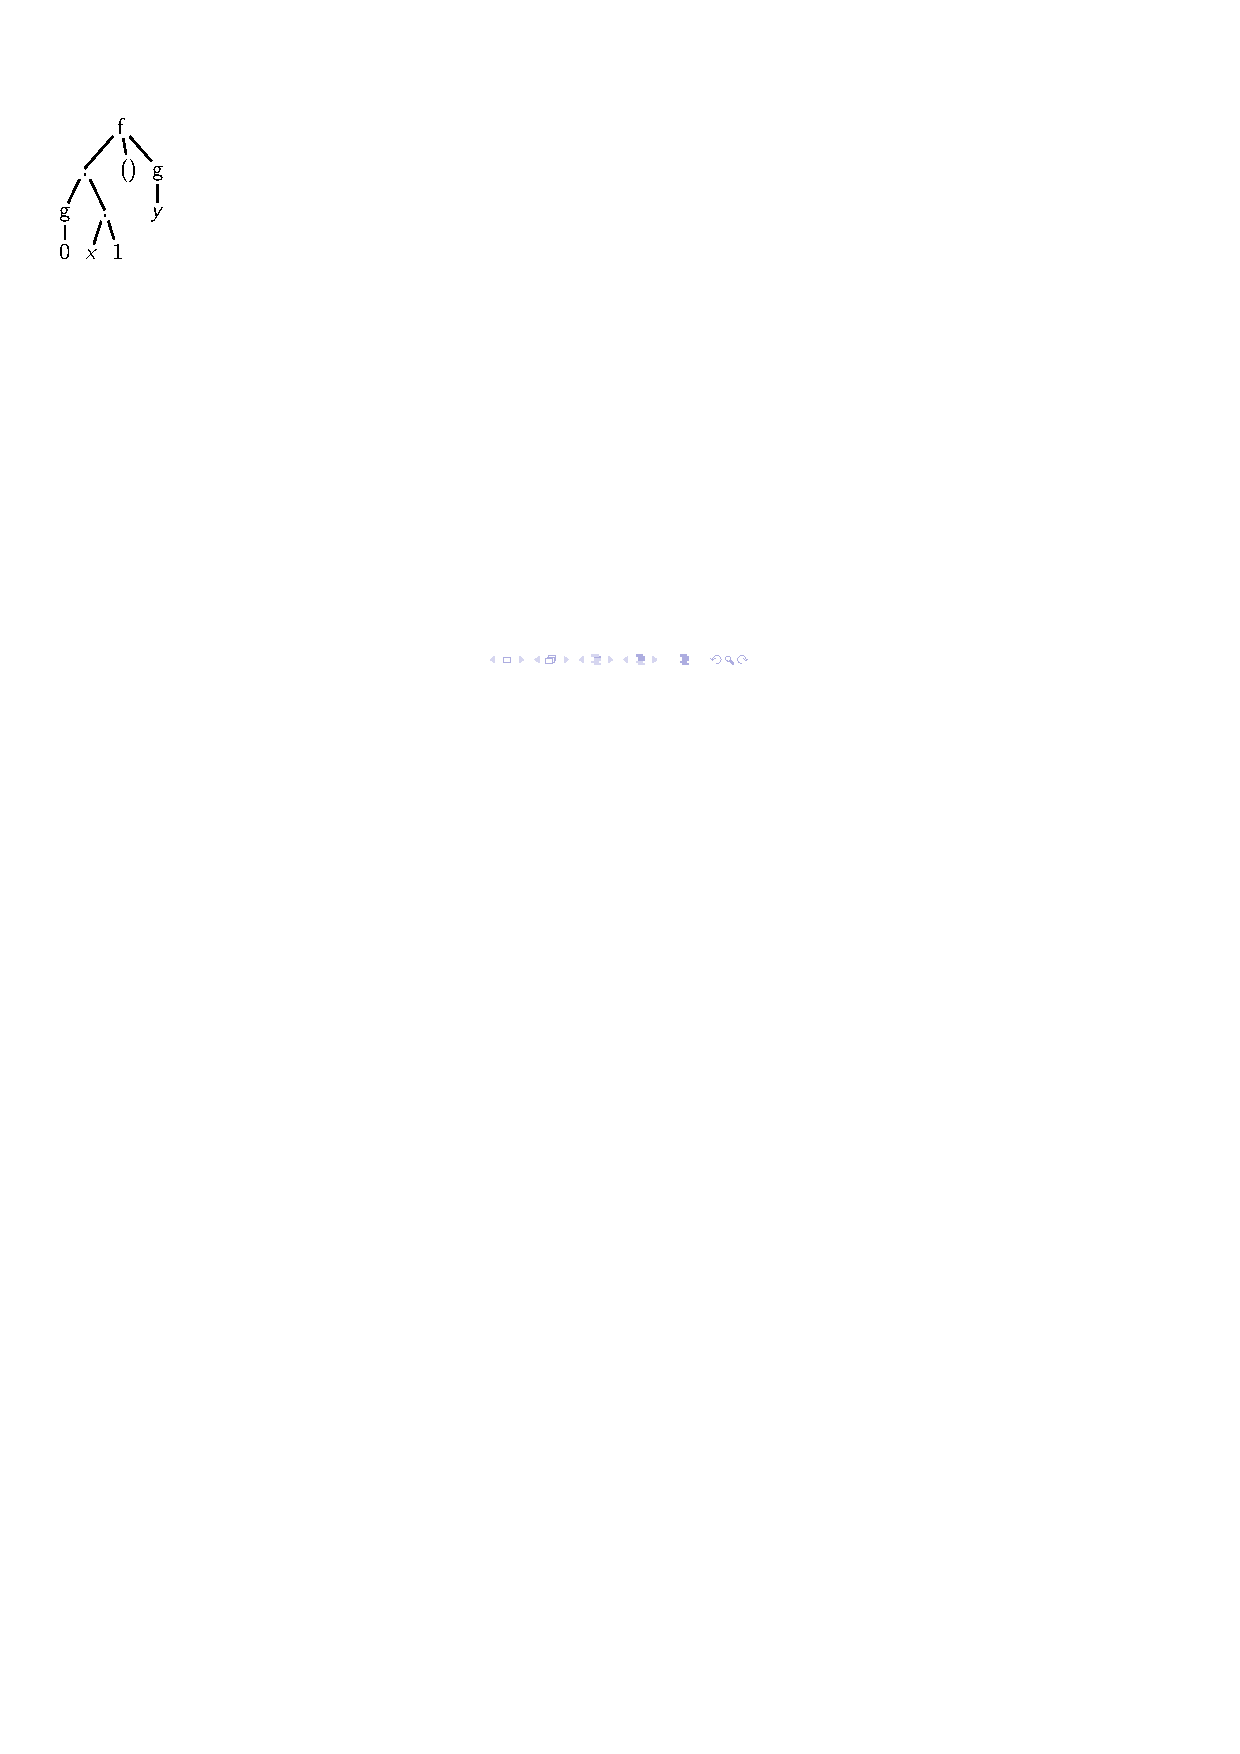
\includegraphics[trim=0 6.2cm 9cm 0]{tree.pdf}
      \end{center}
      is the tree corresponding to the tern
      \(\fun{f}((\fun{g}(0),(x,1)),(),\fun{g}(y))\).

    \item Note that tuples, except the empty tuple, are not
      represented in the tree, since they encode the structure itself,
      which is already laid out. The number of arguments of a function
      is called \textbf{arity}.

  \end{itemize}

\end{slide}

\begin{slide}
  \title{Functional languages}

  \begin{itemize}

    \item For programming, we only consider confluent systems because
      they define partial functions.

    \item To have only one reduction chain per term to the normal
      form, we may also enforce that rules are ordered.

    \item We also enforce that normal forms must be \textbf{values},
      that is, terms without function calls or only with calls to
      functions not occurring on the left\hyp{}hand sides.

    \item In other words, irreducible calls of defined functions are
      not allowed in values.

    \item Systems with these constraints make up a \textbf{functional
      language}.

    \item A program here is a term, and evaluating it means to rewrite
      the term
      \begin{enumerate}
        \item to a value,
        \item or to end in error with a normal form that is not a value,
        \item or to never terminate.
      \end{enumerate}

  \end{itemize}

\end{slide}

\begin{slide}
  \title{Termination}

  \begin{itemize}

    \item We do not require by construction that all functional
      programs terminate, although that is a desirable property, and
      we speak nevertheless of ``functions'' instead of ``partial
      functions'' (which would be technically correct).

    \item If we enforce termination, we loose
      \textbf{Turing\hyp{}completeness}: we cannot program all
      computable functions.

    \item The termination of rewrite systems and, in particular,
      functional programs, is an \textbf{undecidable problem} in
      general.

    \item Nevertheless, there exists a set of well\hyp{}known
      \textbf{decision criteria}, which we will use when programming
      recursive functions in \OCaml.

  \end{itemize}

\end{slide}

\begin{slide}
  \title{Call-by-value}

  \begin{itemize}

    \item If a function call contains at least one other function
      call, there is a choice as to which one to reduce first.

    \item One reduction strategy, named \textbf{call-by-value},
      consists in always reducing the arguments before the call
      itself.

    \item Unfortunately, call-by-value enables otherwise terminating
      rewrites to not terminate. For instance, let us consider
      \begin{equation*}
        \fun{f}(x) \xrightarrow{\alpha} 0\qquad
        \fun{g}() \xrightarrow{\beta} \fun{g}()
      \end{equation*}
      We have \(\fun{f}(\fun{g}()) \xrightarrow{\alpha} 0\)
      but \(\fun{f}(\fun{g}()) \xrightarrow{\beta}
      \fun{f}(\fun{g}()) \xrightarrow{\beta} \dots\)

    \item Despite the loss of expressiveness, we shall retain in this
      lecture the call by value, as it is the strategy of \OCaml and
      it is easy to follow.

    \item In general, the order in which the arguments of a function
      call are evaluated is not specified.

  \end{itemize}

\end{slide}


\begin{slide}
  \title{Call-by-value}

  \begin{itemize}

    \item Another reason to choose call-by-value is that it allows us
      to restrict the shape of the left\hyp{}hand sides, called
      \textbf{patterns}, to one, outermost function call.

    \item For instance, we can then disallow, for being useless, a
      rule like
      \bigskip
      \begin{equation*}
        \fun{plus}(x,\fun{plus}(y,z)) \rightarrow
        \fun{plus}(\fun{plus}(x,y),z).
      \end{equation*}
      \smallskip

      \noindent because, following call\hyp{}by\hyp{}value, the argument
      \(\fun{plus}(y,z)\) must be evaluated before the outermost call,
      therefore it cannot be part of any pattern.

  \end{itemize}

\end{slide}

\begin{slide}
  \title{Higher-order programs, recursion, $\lambda$-calculus}

  \begin{itemize}

    \item Most functional languages allow \textbf{higher\hyp{}order
      function} definitions, whereas standard term\hyp{}rewriting
      systems do not. For example:
      \begin{equation*}
        \fun{f}(g,0) \rightarrow 1
        \qquad
        \fun{f}(g,n) \rightarrow n \times g(g,n-1)
        \qquad
        \fun{fact}(n) \rightarrow \fun{f}(\fun{f},n)
      \end{equation*}
      where \(n \in \mathbb{N}\). Note that these two definitions are
      \textbf{not} recursive, yet the function \fun{fact} is the
      factorial function.

    \item A function definition is \textbf{recursive} if the name of
      the definition occurs on at least one right\hyp{}hand side.

    \item An adequate theoretical framework to understand
      higher\hyp{}order functions is \textbf{\(\lambda\)-calculus}.

    \item In fact, \(\lambda\)-calculus features prominently in the
      semantics of programming languages, even not functional ones.

    \item For didactic purposes, we began with rewrite systems because
      they offer implicit pattern matching (that is, rule selection).

  \end{itemize}

\end{slide}

\begin{slide}
  \title{Stacks in a functional setting}

  \begin{itemize}

    \item We show how to express linear data structures in a purely
      functional language and how to compute with them.

    \item The simplest of those structures is the \textbf{stack}.

    \item A stack can be thought of as a finite series of items that
      can only be accessed sequentially from one end, called the
      \textbf{top}, following the analogy with a stack of material
      objects.

  \end{itemize}

\end{slide}
\begin{slide}
  \title{Stacks in a functional setting (continued)}

  \begin{itemize}

    \item To define a stack in a functional language, one uses calls
      to undefined functions to model all the possible shapes a stack
      can take.

    \item Here, a stack can be either empty or not.

    \item Let \(\fun{nil}()\) be the irreducible call that denotes an
      empty stack (the function \fun{nil} is undefined).

    \item If not empty, the stack then must contain a topmost (first)
      item, and a \textbf{substack}, that is, the stack made of all
      the items but the first.

    \item Let \(\fun{cons}(x,s)\) denote the non\hyp{}empty stack with
      the item~\(x\) on top and the \textbf{immediate substack}~\(s\).

  \end{itemize}

\end{slide}

\begin{slide}
  \title{Inductive definition of stacks}

  \begin{itemize}

    \item The previous definition is intuitive, but not formal yet.

    \item Data structures are usually defined \textbf{inductively}.

    \item Let~\(\mathcal{T}\) be the set of all possible terms and
      \(\mathcal{S} \subset \mathcal{T}\) be the set of all stacks.

    \item Formally, \(\mathcal{S}\)~can by defined by
      \textbf{induction} as the smallest set such that
      \begin{enumerate}

        \item \(\fun{nil}() \in \mathcal{S}\);

        \item if \(x \in \mathcal{T}\) and \(s \in \mathcal{S}\), then
          \(\fun{cons}(x,s) \in \mathcal{S}\).
      \end{enumerate}

    \item We take the smallest set because we do not want
      in~\(\mathcal{S}\) terms that were not constructed by the
      inductive rules (this is called the \textbf{smallest fixed
        point} of the inductive relation).

  \end{itemize}

\end{slide}

\begin{slide}
  \title{Appending a stack}

  \begin{itemize}

    \item For all \(s, t \in \mathcal{S}\), let us consider the
      functional program
      \bigskip
      \begin{align*}
        \fun{cat}(\fun{nil}(),t) &\xrightarrow{\alpha} t\\
        \fun{cat}(\fun{cons}(x,s),t) &\xrightarrow{\smash\beta}
        \fun{cons}(x,\fun{cat}(s,t))
      \end{align*}
      \smallskip

    \item This is a functional program suitable for
      call\hyp{}by\hyp{}value reduction strategy, because the function
      calls in the patterns (i.e., left\hyp{}hand sides) are
      irreducible.

    \item The right\hyp{}hand sides are stacks, so a call to
      ``\fun{cat}'' is a stack.

    \item Rule~\(\alpha\) says that, if the first stack is empty, the
      value is the second.

    \item In rule~\(\beta\), the first stack is not empty, and its top
      item is the top of the final stack (\(x\)), the immediate
      substack (\(s\)) being used in a call to ``\fun{cat}'' with the
      second stack (\(t\)) unchanged.

  \end{itemize}

\end{slide}

\begin{slide}
  \title{Appending a stack}

  \begin{itemize}

    \item This function appends the second stack at the bottom of a
      \textbf{copy} of the first. (The function name ``\fun{cat}''
      stands for ``catenation'', and is slightly better than
      ``\fun{app}'').

    \item We could also say that this function appends a copy of the
      first stack on top of the other. But this is not the same as
      pushing the first stack on top of the other, like
      \bigskip
      \begin{equation*}
        \fun{cat}(s,t) \rightarrow \fun{cons}(s,t) \qquad
        \text{Wrong!}
      \end{equation*}
      \smallskip

    \item This is \textbf{not} appending: here, the stack~\(s\)
      becomes an item of the resulting stack, but we want only the
      \textbf{contents} of~\(s\) to be pushed on top of~\(t\), not
      their container.

    \item Analogy: You may think of an empty stack as a empty
      cardboard box, open topside, and every item pushed in it is like
      a book that you put on the topmost book, or at the bottom of the
      box if this is the first book.

  \end{itemize}

\end{slide}


\begin{slide}
  \title{Appending a stack}

  \begin{itemize}

    \item Let us set the abbreviations
      \begin{itemize}

        \item \(\el := \fun{nil}()\),

        \item \(\cons{x}{s} := \fun{cons}(x,s)\),

      \end{itemize}
      after the convention of the programming language \OCaml.
      \medskip

    \item We can further abbreviate
      \begin{itemize}

        \item \(\cons{x_1}{\cons{x_2}{\cons{\dots}{\cons{x_n}{s}}}} :=
          \fun{cons}(x_1, \fun{cons}(x_2, \dots \fun{cons}(x_n,s)))\)

        \item \([x] := \cons{x}{\el}\)

        \item \([x_1; x_2, \dots; x_n] :=
          \cons{x_1}{\cons{x_2}{\cons{x_3}{\cons{\ldots}{\cons{x_n}{\el}}}}}\).
      \end{itemize}
      \medskip

    \item Our system now becomes a bit more legible:
      \bigskip
      \begin{align*}
        \fun{cat}(        \el,t) &\xrightarrow{\alpha} t\\
        \fun{cat}(\cons{x}{s},t) &\xrightarrow{\smash{\beta}}
        \cons{x}{\fun{cat}(s,t)}
      \end{align*}

  \end{itemize}

\end{slide}

\begin{slide}
  \title{Pattern matching}

  \begin{itemize}

    \item Let us compute \(\fun{cat}([1;2],[3])\).

    \item We need to find the first rule that is matched by this call.

    \item Remember that the arguments must be values before you do
      that.

    \item Intuitively, this means that we compare the call with the
      patterns, that is, the left\hyp{}hand sides of the rules, in
      order.

    \item Here, rule~\(\alpha\) is not matched because \([1;2] \neq
      []\).

    \item Rule~\(\beta\) is matched because \([1;2] = 1::[2]\) and
      equals the sub\hyp{}pattern \(x::s\) if we assign \(x := 1\) and
      \(s := [2]\). Also, trivially, \(t := [3]\) works.

    \item After the rule~\(\beta\) is selected, the assignments are
      used to replace the variables in the right\hyp{}hand sides.

    \item The whole evaluation is
    \begin{equation*}
      \fun{cat}([1;2],[3])
      \xrightarrow{\beta}
      \cons{1}{\fun{cat}([2],[3])}
      \xrightarrow{\beta}
      \cons{1}{\cons{2}{\fun{cat}(\el,[3])}}
      \xrightarrow{\alpha}
                    [1;2;3].
    \end{equation*}
  \end{itemize}

\end{slide}

\begin{slide}
  \title{Abstract syntax trees}

  \begin{itemize}

    \item Depending on the context, we may use the arborescent
      depiction of terms to bring to the fore certain aspects of a
      computation.

    \item For example, it may be interesting to show how parts of the
      output (the right\hyp{}hand side) are actually \textbf{shared}
      with the input (the left\hyp{}hand side).

    \item In other words, how much (new) data is created by a given
      rule.

    \item This concept supposes that terms reside in some sort of
      space and that they can be referred to from different other
      terms.

    \item This abstract space serves as a model of an interpreter's
      memory, called the \textbf{heap}.

  \end{itemize}

\end{slide}

\begin{slide}
  \title{Data sharing}

  \begin{itemize}

    \item Consider for instance
      \begin{center}
        \centering
        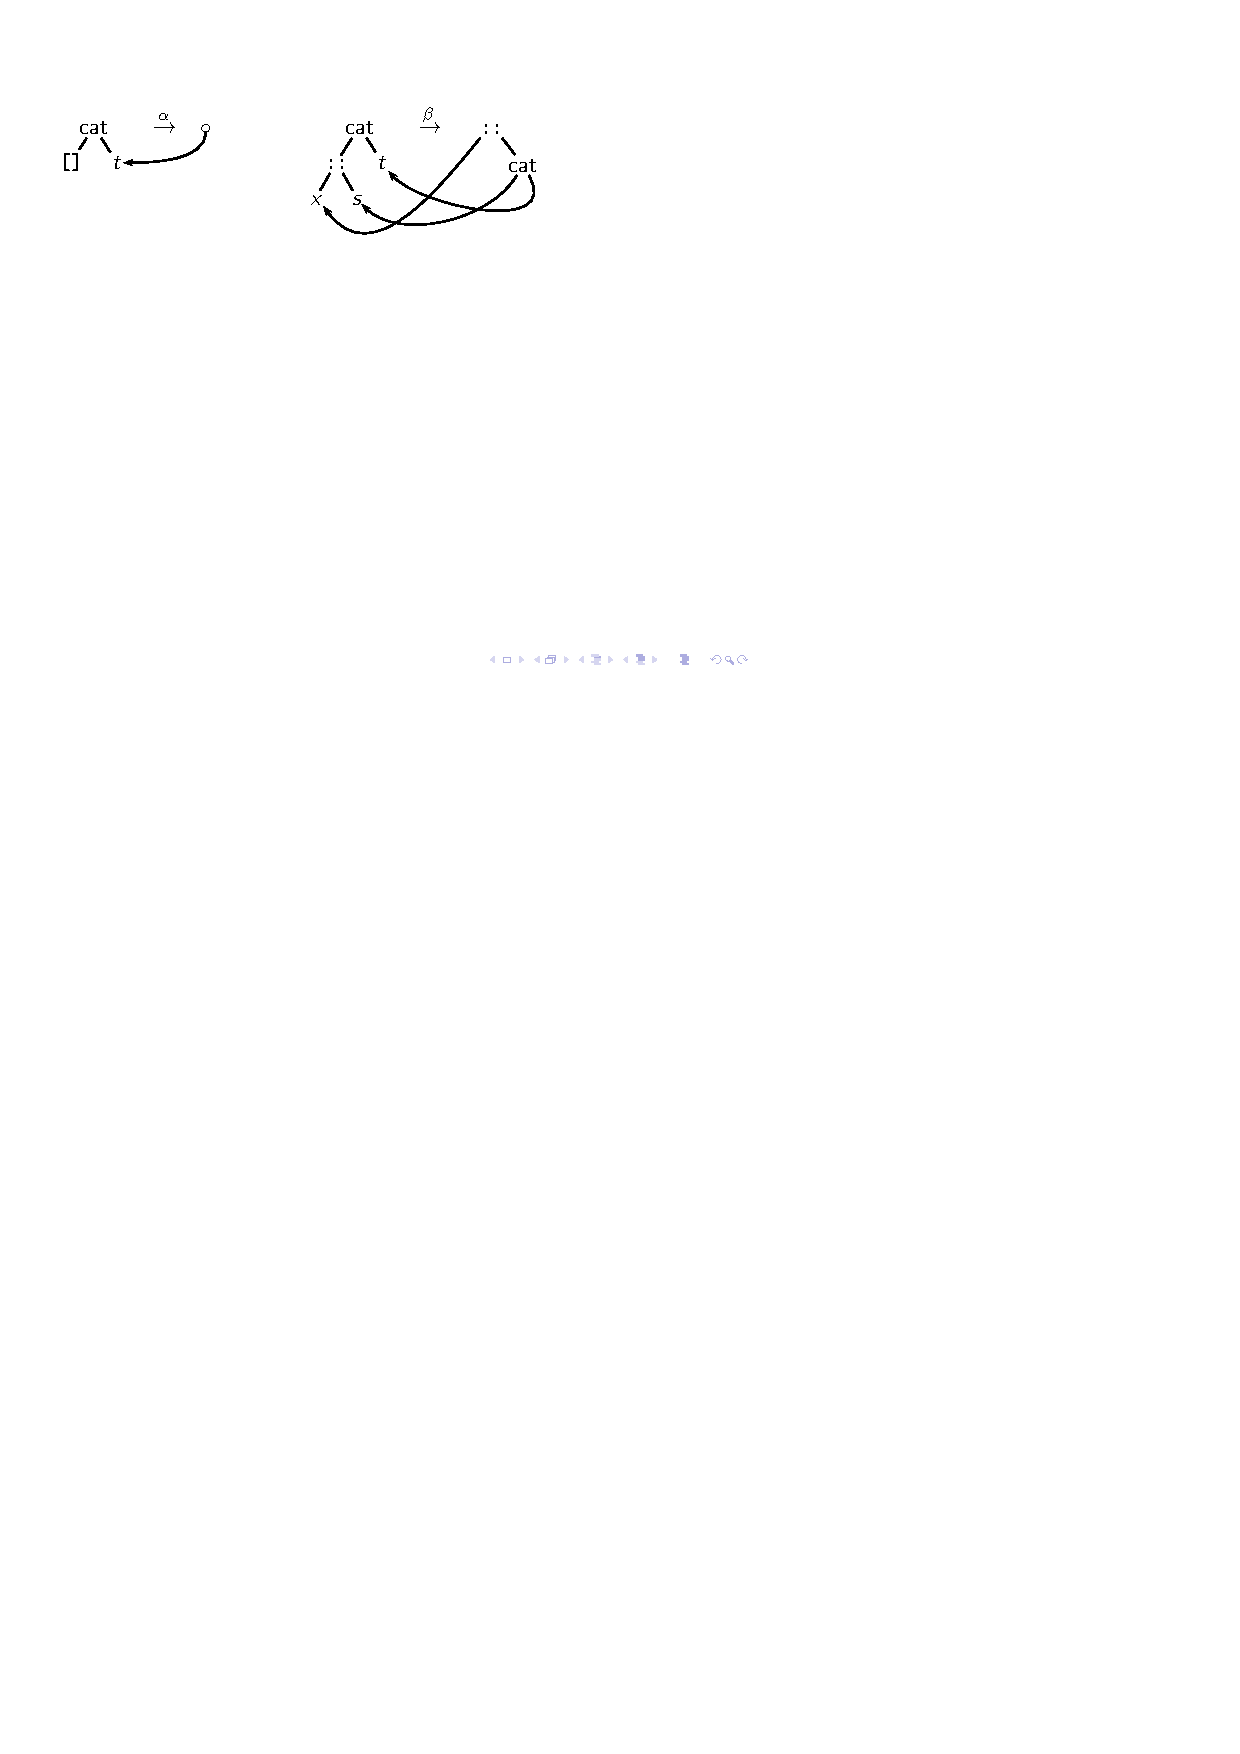
\includegraphics[trim=0 7cm 5cm 0]{cat_dag.pdf}
        \bigskip
      \end{center}
      which is the same definition of ``\fun{cat}'' as given above:
      \bigskip
      \begin{equation*}
        \fun{cat}(\el,t) \xrightarrow{\alpha} t
        \qquad\qquad\qquad
        \fun{cat}(\cons{x}{s},t) \xrightarrow{\beta}
        \cons{x}{\fun{cat}(s,t)}
      \end{equation*}
      \smallskip

    \item The arrows on certain edges denote data sharing.

    \item When trees are used to visualise terms, they are called
      \textbf{abstract syntax trees} (AST).

    \item When some trees share subtrees, the whole \textbf{forest}
      (set of trees) is called a \textbf{directed acyclic graph}
      (DAG).

  \end{itemize}

\end{slide}

\begin{slide}
  \title{Data sharing and evaluation}

  \begin{itemize}

    \item The evaluation of \(\fun{cat}([1;2],[3])\) is:
      \bigskip
      \begin{center}
        \includegraphics{cat123_push.eps}
      \end{center}

  \end{itemize}

\end{slide}

\begin{slide}
  \title{Data sharing and evaluation}

  \begin{itemize}

    \item Note that each right-hand side shows only the rewritten
      call, not the whole term.

    \item Therefore, to reconstruct the value, we need to work
      leftwards and replace the rewritten call by the right-hand side:
      \medskip
      \begin{center}
        \includegraphics{cat123_pop0.eps}
        \bigskip
      \end{center}

    \item We do not show the calls that have been replaced by their
      values.

  \end{itemize}

\end{slide}

\begin{slide}
  \title{Data sharing and evaluation}

  \begin{center}
    \includegraphics{cat123_pop1.eps}
    \qquad\quad
    \includegraphics{cat123_pop2.eps}
  \end{center}

\end{slide}

\begin{slide}
  \title{Call stack}

  \begin{itemize}

    \item We can see that the value of the second argument, [3], is
      shared with the value of the call, as well as the integers~1
      and~2.

    \item We saw how rewrites accumulated rightwards until the result
      had to be reconstructed by replacing leftwards the right-hand
      sides.

    \item This dynamic is that of a stack, but a stack holding
      suspended function calls (that is, awaiting their values) and
      references to ASTs in the heap.

    \item This is the \textbf{call stack}.

    \item The top of the stack (here, the rightmost abstract syntax
      tree) is the next term to be rewritten, unless the call on the
      left\hyp{}hand side is the original call, in which case the top
      is its value.

  \end{itemize}

\end{slide}

\begin{slide}
  \title{Garbage collection}

  \begin{itemize}

    \item In the abstract syntax trees (AST), the nodes with the calls
      that are replaced by their values have been immediately removed.

    \item In fact, they could have been removed later, in any order.

    \item The process which identifies and discards useless ASTs is
      called the \textbf{garbage collector} (GC).

    \item A term is useless if it cannot be accessed from anywhere in
      the call stack.

    \item Contrary to the heap, which can be thought of as an
      unordered set of trees (a forest of DAGs), the call stack is an
      ordered set that can be efficiently extended or reduced.

    \item The garbage collector can be conceived as a process
      interleaved with the process of evaluation.

    \item Like evaluators of functional programs, garbage collectors
      may also have different strategies (as to when dispose of
      useless data).
  \end{itemize}

\end{slide}

\begin{slide}
  \title{Tail call optimisation}

  \begin{itemize}

    \item Let us define a function that sums integers in a
      non\hyp{}empty list:
      \begin{equation*}
        \fun{sum}([n]) \xrightarrow{\alpha} n\qquad
        \fun{sum}(\cons{n}{s}) \xrightarrow{\beta} n + \fun{sum}(s)
      \end{equation*}

    \item The view of the system with maximum sharing is:
      \begin{center}
        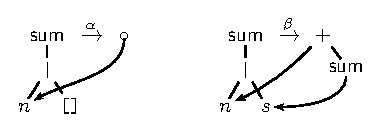
\includegraphics{sum_dag.eps}
      \end{center}

  \end{itemize}

\end{slide}

\begin{slide}
  \title{Tail call optimisation}

  The first phase of the evaluation of \(\fun{sum}([3;7;5])\) is:
  \begin{center}
    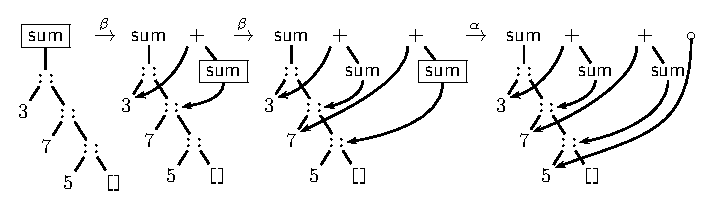
\includegraphics[scale=1]{sum375_push.eps}
  \end{center}

\end{slide}

\begin{slide}
  \title{Tail call optimisation}

  The second phase (replacing the pending calls with their values) is
  \begin{center}
    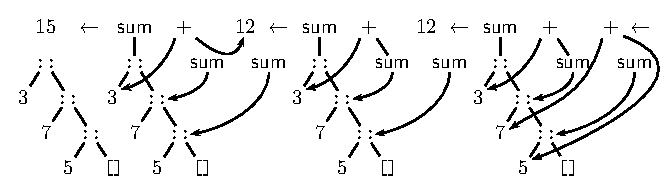
\includegraphics[scale=1]{sum375_pop.eps}
  \end{center}

\end{slide}

\begin{slide}
  \title{Tail call optimisation}

  The same, with a garbage collector that collects after each
  replacement:
  \begin{center}
    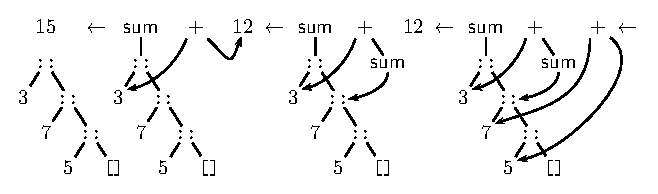
\includegraphics[bb=149 585 416 661]{sum375_pop1.eps}
  \end{center}

\end{slide}

\begin{slide}
  \title{Tail call optimisation}

  \begin{itemize}

    \item Let us consider an alternate version of \fun{sum}:
      \begin{equation*}
        \begin{array}{@{}r@{\;}l@{\;}l@{}}
          \fun{sum}_1(\cons{n}{t}) & \xrightarrow{\gamma}
          & \fun{sum}_0(n,t).\\
          \fun{sum}_0(n,\el) & \xrightarrow{\delta} & n\\
          \fun{sum}_0(n,\cons{m}{s}) & \xrightarrow{\epsilon}
          & \fun{sum}_0(n+m,s).
        \end{array}
      \end{equation*}

    \item For \(\fun{sum}_1([3;7;5])\) we have the evaluation
      \begin{center}
        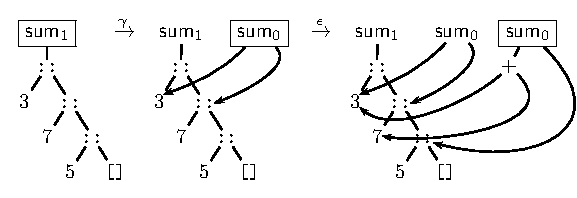
\includegraphics[bb=71 630 356 721]{sum0_375_0.eps}
      \end{center}

  \end{itemize}

\end{slide}

\begin{slide}
  \title{Tail call optimisation}

  \begin{center}
    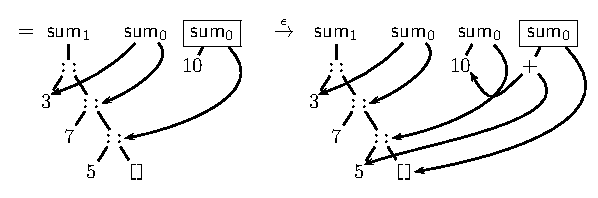
\includegraphics[bb=71 626 352 721]{sum0_375_1.eps}
    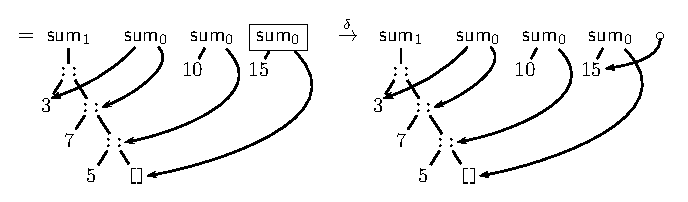
\includegraphics[bb=71 636 394 721]{sum0_375_2.eps}
  \end{center}

\end{slide}

\begin{slide}
  \title{Tail call optimisation}

  \begin{itemize}

    \item Notice that, in the case of \fun{sum}$_0$, we found the
      result (15) at the end of the first phase (of growing the call
      stack).

    \item Therefore, there is no need for a second phase, which
      replaces the pending calls by their values: we can discard all
      those calls at once after the first phase.

    \item Or, to see it even more clearly, let us rewrite the same
      first phase and assume that the collector reclaims immediately
      the useless pending calls:
      \begin{center}
        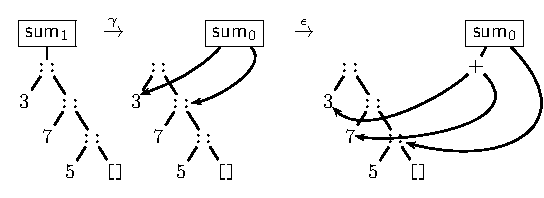
\includegraphics[bb=71 628 327 721]{sum0_375tco0.eps}
      \end{center}

  \end{itemize}

\end{slide}

\begin{slide}
  \title{Tail call optimisation}

  \begin{center}
    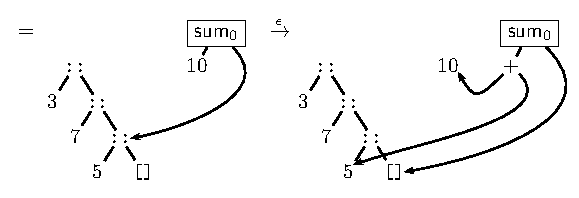
\includegraphics[bb=71 628 350 721]{sum0_375tco1.eps}
    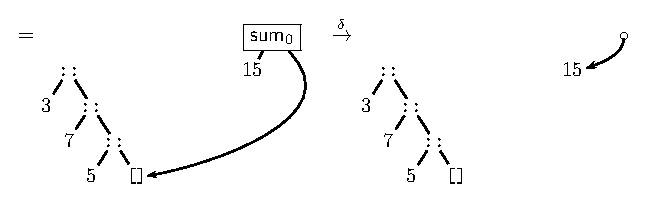
\includegraphics[bb=71 636 375 721]{sum0_375tco2.eps}
  \end{center}

\end{slide}

\begin{slide}
  \title{Tail call optimisation}

  \begin{itemize}

    \item As we see now, we can keep the size of the call stack
      constant, if we reclaim the top at each new rewrite.

    \item This optimisation is called \textbf{tail call optimisation}.

    \item Intuitively, a call in \textbf{tail position} is a call
      whose value is the value of the previously rewritten call.

    \item For example, the call \(f(x)\) in \(1 + f(x)\) is not in
      tail position, because its value needs to be incremented.

    \item Most compilers of functional languages detect and implement
      that optimisation that saves memory.

    \item Even the \Clang compiler of \textsf{GCC}.

  \end{itemize}

\end{slide}


\end{document}
